\section{Базовые морфологические операции}
\subsection{Исходное изображение}

Для первого задания выберем фотографию Яна Берри, сделанную в разгар событий Пражской весны:
\begin{figure}[ht!]
    \centering
    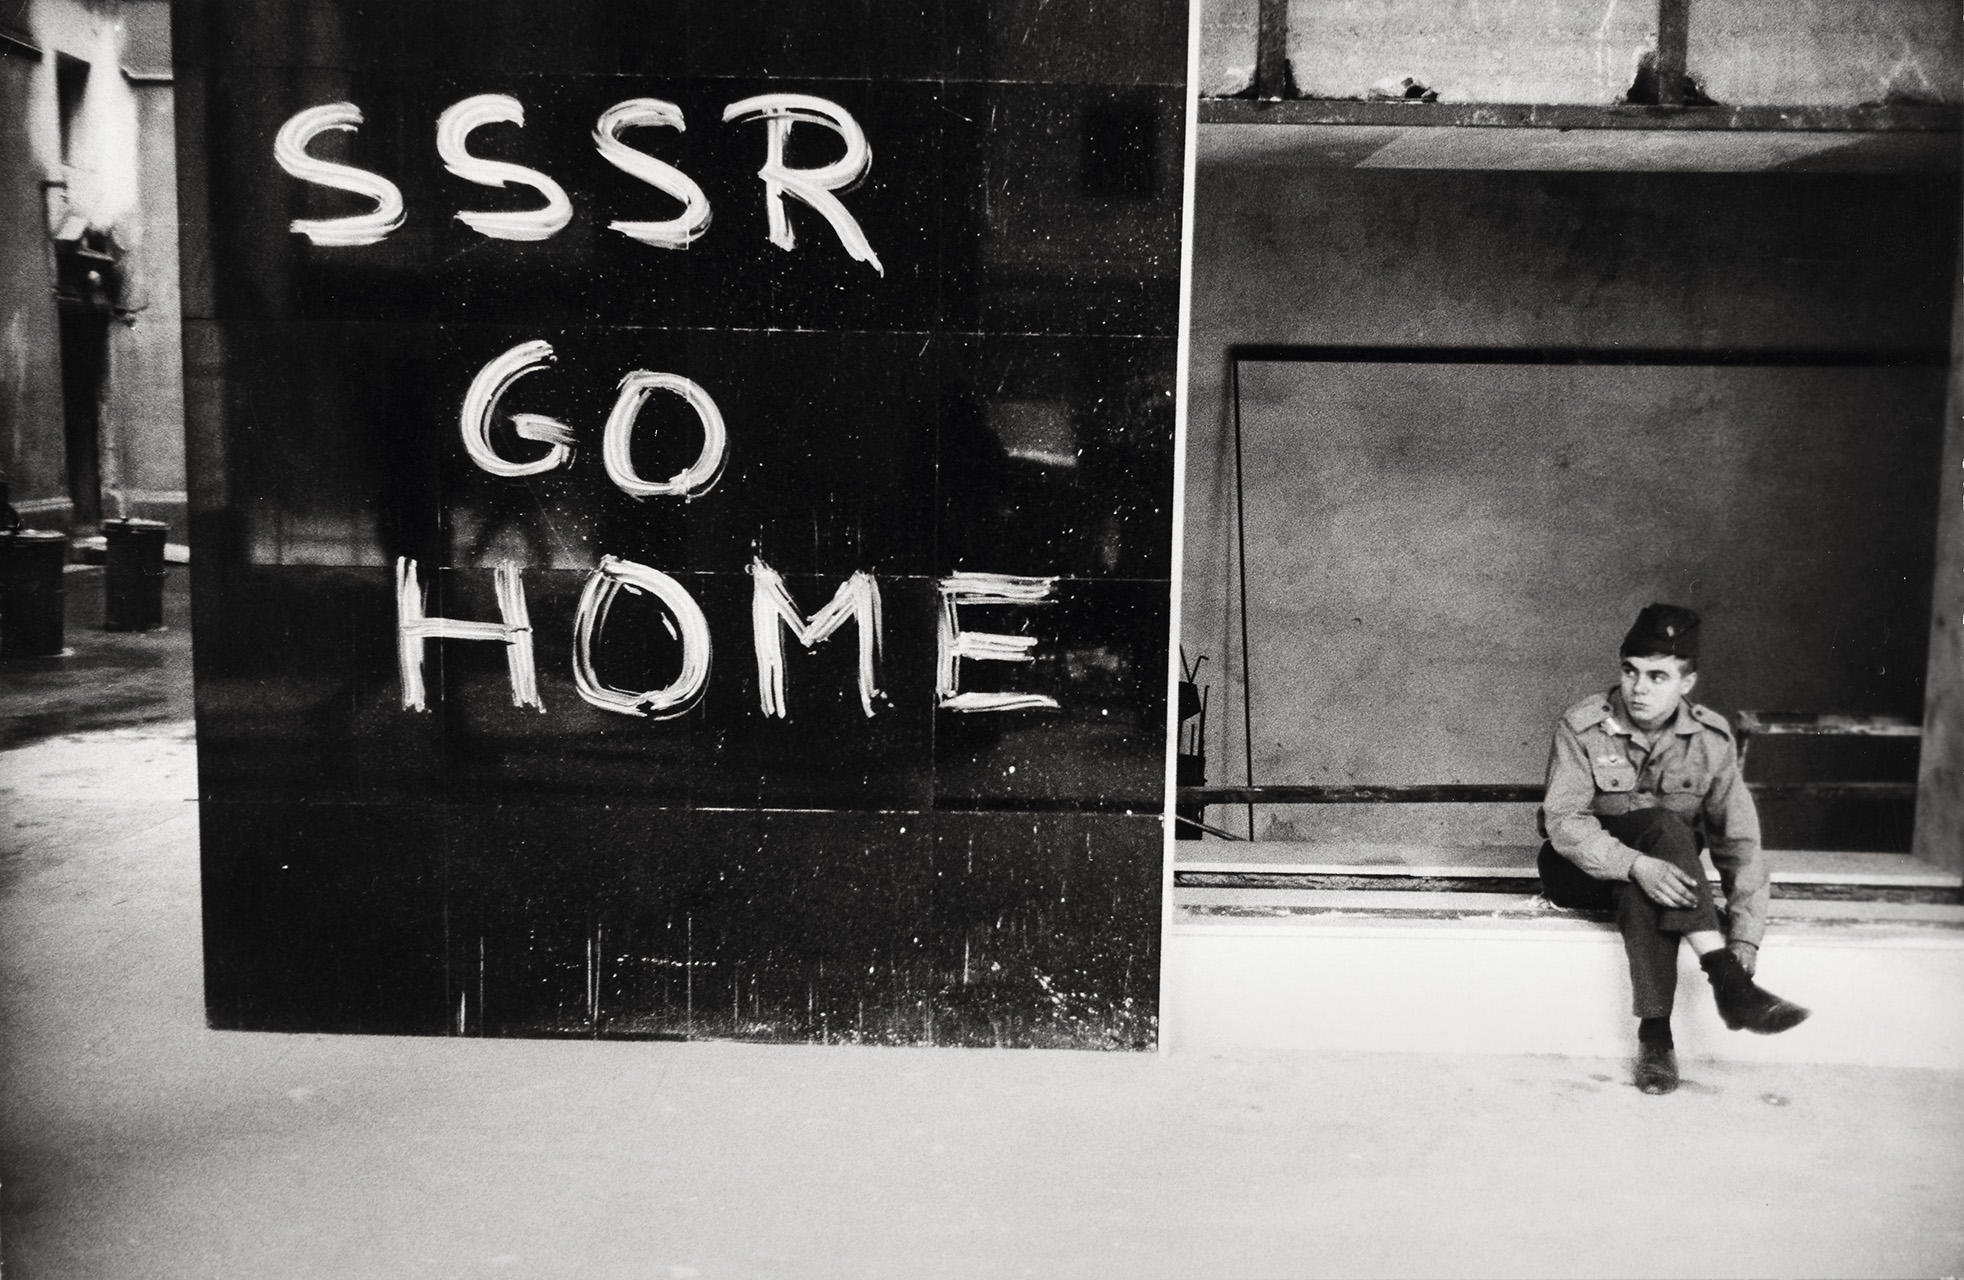
\includegraphics[width=\textwidth]{images/source_images/Ian_Berry_A young_Russian soldier.jpg}
    \caption{Ян Берри. Молодой советский солдат отдыхает рядом с плакатом <<СССР, возвращайся домой>> на Вацлавской площади. Прага, Чехословакия. 1968}
    \label{img:Soldier_orig}
\end{figure} 

Нашей задачей будет минимизация дефектов формы на надписи \textit{SSSR GO HOME}. В этом нам поможет \textit{Python}. Для начала загрузим изображение и выберем область изображения с надписью для выполения преобразований.

\begin{lstlisting}[caption={Исходный код для считывания изображения}, label={lst:img_reading}]
    # loading grayscale image
    src_img = cv.imread('source_images/Ian_Berry_A young_Russian soldier.Jpeg', 0)
    assert src_img is not None, "File could not be read"
    result = np.copy(src_img)
    # selecting specific area
    spec_area = src_img[0:735, 200:1080]
\end{lstlisting}

\begin{figure}[ht!]
    \centering
    
\includegraphics[width=0.7\textwidth]{images/transformed_images/1/Caption.jpg}
    \caption{Надпись, которая подвергнется преобразованиям}
    \label{img:Caption_orig}
\end{figure} 

С помощью эрозии избавимся от лишних точек на стене и выступов на буквах. Далее применим дилатацию от избавления от <<внутренних дырок>> и затем эрозию для избавления от частиц, появившихся в результате дилатации, и возвращения буквам их исходной толщины.

\begin{lstlisting}[caption={Исходный код для преобразования надписи}, label={lst:morphological}]
    # morphological operations
    disk = cv.getStructuringElement(cv.MORPH_ELLIPSE, (3, 3))
    erosion = cv.erode(spec_area, disk, iterations=1)
    dilation = cv.dilate(erosion, disk, iterations=7)
    erosion2 = cv.erode(dilation, disk, iterations=5)
\end{lstlisting}
\begin{figure}
    \centering
    \begin{subfigure}[b]{0.3\textwidth}
        \centering
        
\includegraphics[width=\textwidth]{images/transformed_images/1/4 try/Erosed_1.jpg}
        \caption{}
        \label{img:Caption_erosed_1}
    \end{subfigure}
    \begin{subfigure}[b]{0.3\textwidth}
        \centering
        
\includegraphics[width=\textwidth]{images/transformed_images/1/4 try/Dilation_7.jpg}
        \caption{}
        \label{img:Caption_dilation}
    \end{subfigure}
    \begin{subfigure}[b]{0.3\textwidth}
        \centering
        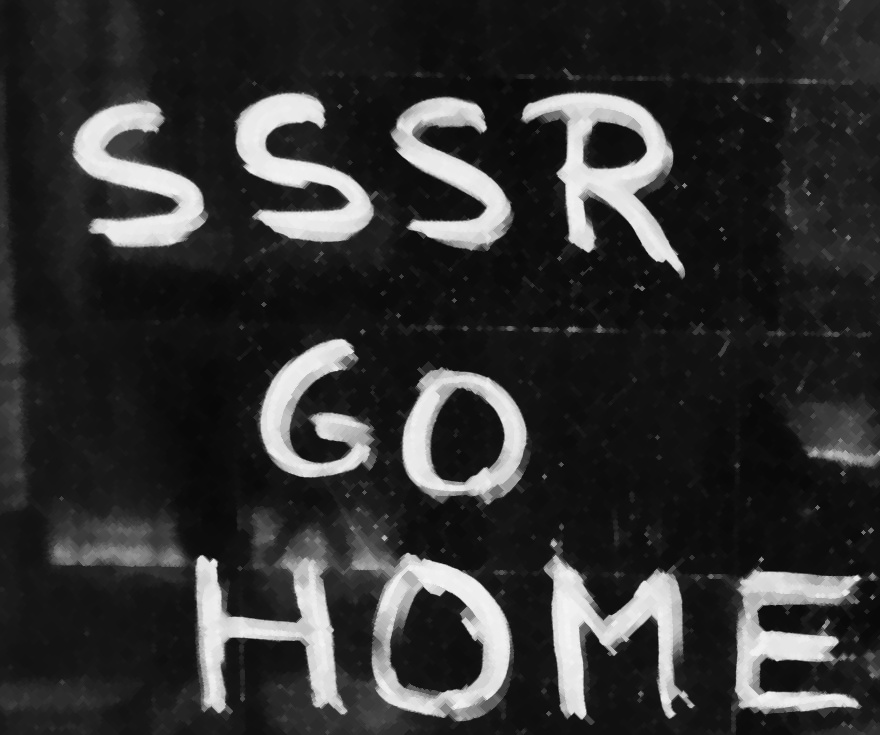
\includegraphics[width=\textwidth]{images/transformed_images/1/4 try/Erosed_2_5.jpg}
        \caption{}
        \label{img:Caption_erosed_2}
    \end{subfigure}
    \caption{Избавление от дефектов: (а) результат применения эрозии, (b)  результат применения дилатации 7 раз, (c)  результат применения эрозии 5 раз}
    \label{img:Transforms}
\end{figure}
\clearpage

\subsection{Результаты}

После преобразований необходимо вернуть <<новую>> надпись в исходное изображение.

\begin{lstlisting}[caption={Исходный код для получения итогового изображения}, label={lst:result}]
    # displaying transformed image
    result[0:735, 200:1080] = erosion2
    display_image('Result', result, 1)
\end{lstlisting}

\begin{figure}[ht!]
    \centering
    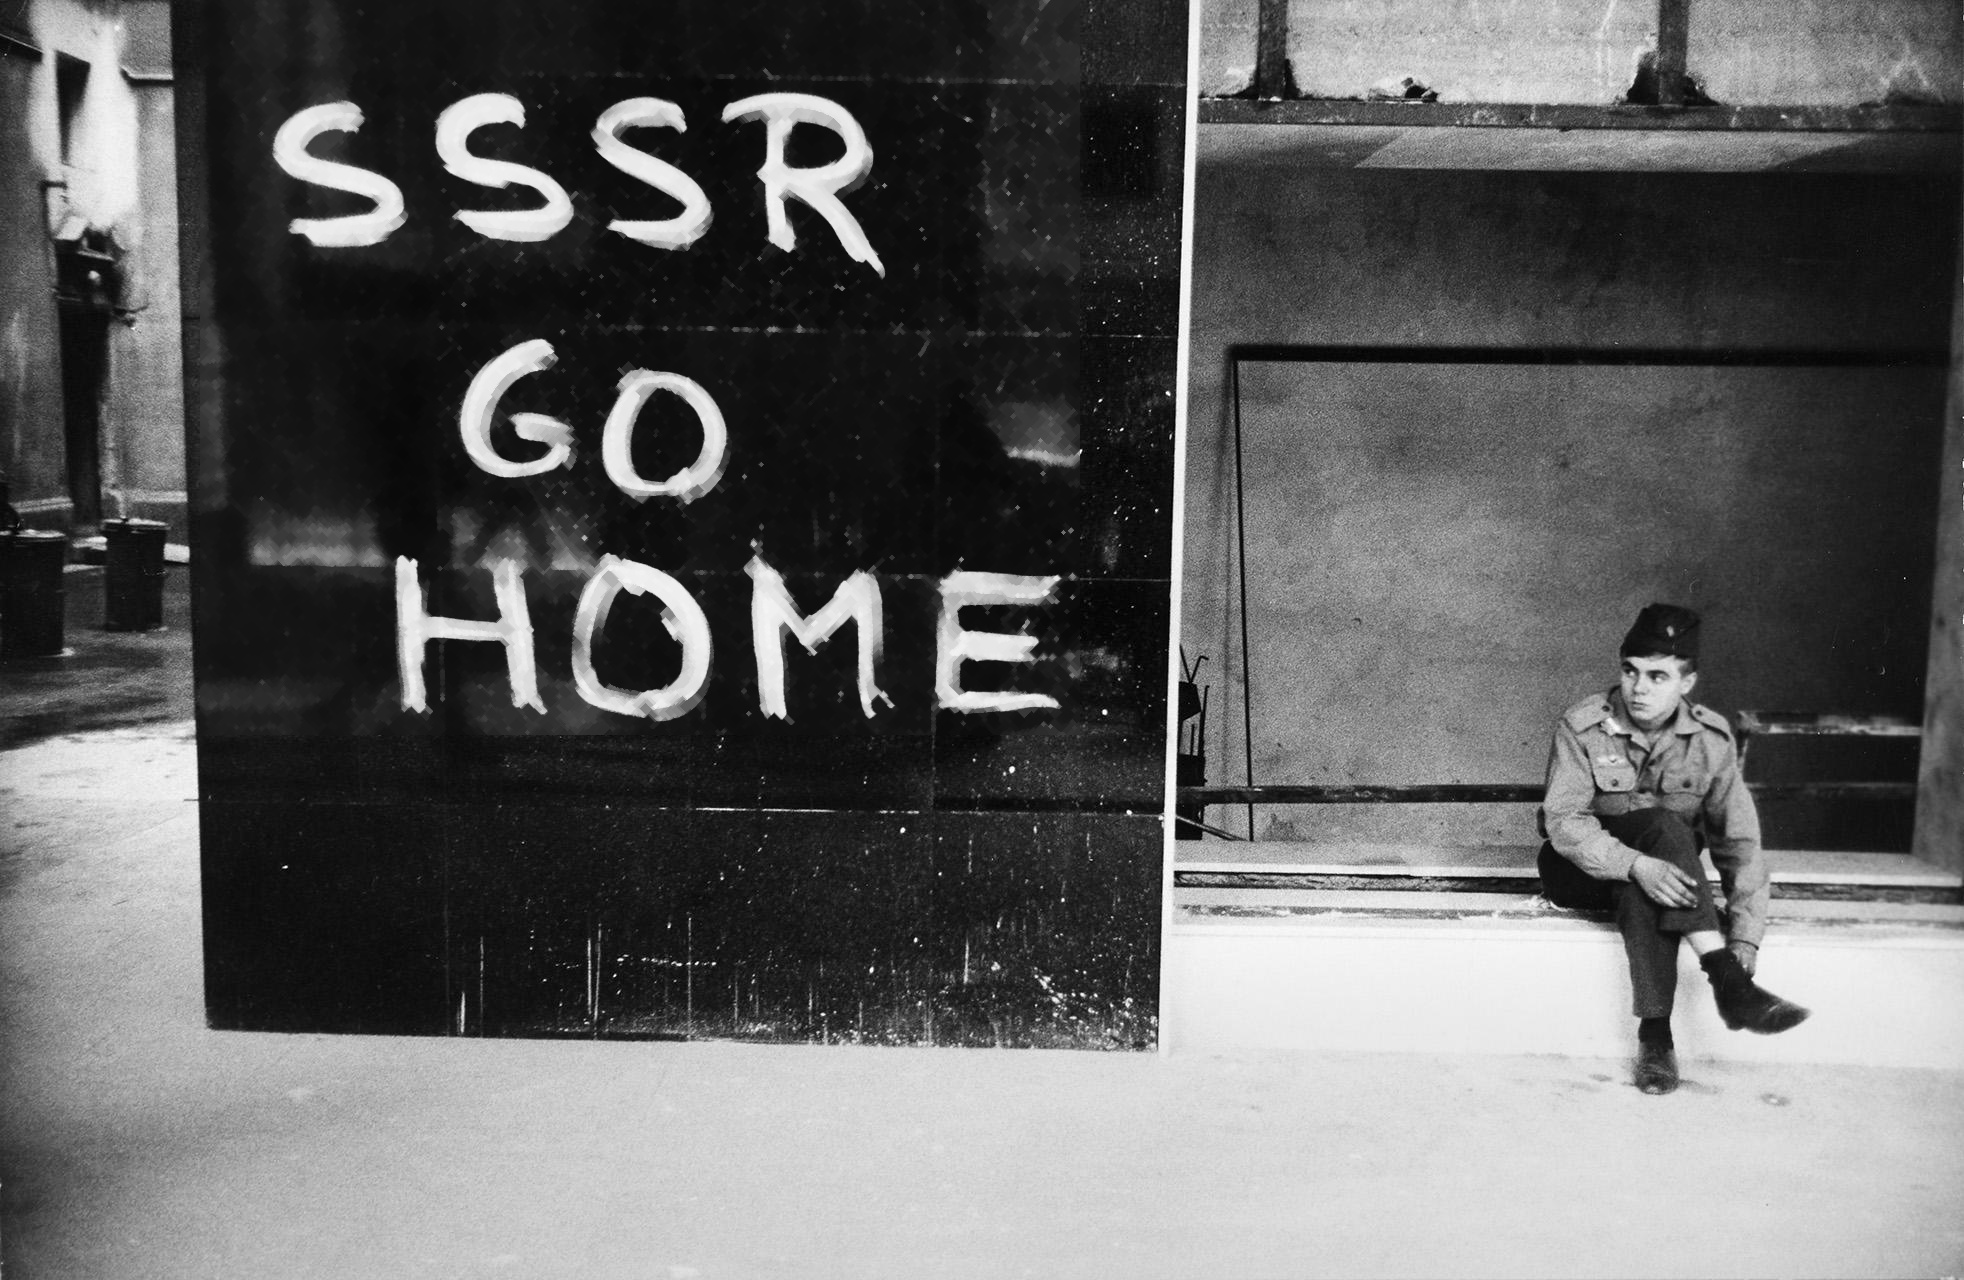
\includegraphics[width=\textwidth]{images/transformed_images/1/4 try/Result.jpg}
    \caption{Результат применения базовых морфологических операций}
    \label{img:Soldier_result}
\end{figure} 



\newpage
\section{Разделение объектов}
\subsection{Исходное изображение}

Обратимся к кругам и их производным. Исходное изображение:

\begin{figure}[ht!]
    \centering
    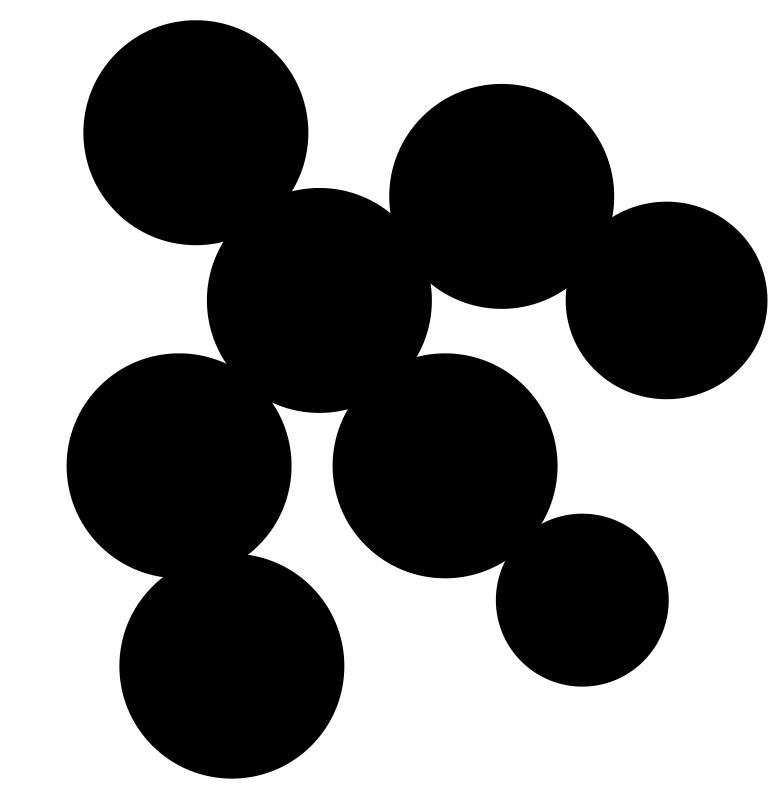
\includegraphics[width=0.5\textwidth]{images/source_images/circles.jpg}
    \caption{Круги}
    \label{img:circles_orig}
\end{figure} 

Для выполнения этого задания воспользуемся \textit{MATLAB}.

\subsection{Программа на языке MATLAB}

\begin{lstlisting}[caption={Исходный код программы для разделения объектов}, label={lst:separation}]
    src_img = imread("circles.jpg");
    gray_img = im2gray(src_img);
    BW = imbinarize(gray_img);
    BW = ~BW;
    imwrite(BW,"binary_inv.jpg");
    BW2 = bwmorph(BW,'erode',45);
    imwrite(BW,"erosed.jpg");
    BW2 = bwmorph(BW2,'thicken',Inf);
    imwrite(BW,"boundaries.jpg");
    BW = ~(BW & BW2);
    imwrite(BW,"result.jpg");
\end{lstlisting}

\subsection{Результаты}

\newpage
\section{Сегментация}

\newpage
\section{Выводы}

В результате выполнения работы мы познакомились с преобразованием Хафа для поиска геометрических примитивов.

Стоит отметить, что важную роль в успешном определении прямых линий и окружностей играет оператор Кэнни, который обнаруживает контуры изображения. Нам удалось убедиться в этом при использовании полутонового изображения для преобразования Хафа: результаты при обнаружении прямых были удручающими (см. рисунки \ref*{img:fin_ITMO_gray}, \ref*{img:fin_fir_gray} и \ref*{img:fin_piet_gray}), а при определении окружностей программа не смогла ничего вывести.

Полный код программы и изображения можно найти на \href{https://github.com/NikBrat/ComputerVision_Lab5}{GitHub}.

\section{Ответы на вопросы}

\newcounter{question}
\setcounter{question}{0}

\newcommand{\question}[1]{\item[Q\refstepcounter{question}\thequestion.] #1}
\newcommand{\answer}[1]{\item[A\thequestion.] #1}


\begin{itemize}

    \question{Какая идея лежит в основе преобразования Хафа?}
   
    \answer{ В основе данного преобразования лежит идея поиска общего геометрического места точек (ГМТ) с помощью метода <<голосования>> точек. В классическом преобразовании также используется идея пространства параметров $(\theta, \rho)$ уранения прямой $y=kx+b$ $\Leftrightarrow$ $xcos(\theta)+ysin(\theta)=\rho$}
    
    \question{Можно ли использовать преобразование Хафа для поиска произвольных контуров, которые невозможно описать аналитически?}
    \answer{Решение данной задачи возможно при использовании \textbf{обобщеннго преобразования Хафа}.} 

    \question{Что такое рекуррентное и обобщенное преобразования Хафа?}
    \answer{Особенность рекуррентного преобразования Хафа заключается в том, что мы применяем преобразование в скользящем окне, определяя аккумулятор преобразования для каждой области, после чего будем составлять общий аккумуляторный массив. В результате каждая точка общего аккумулятора будет характеризоваться параметрами наиболее достоверного отрезка прямой, проходящего через него.
    
    Обобщенное преобразование Хафа применяется для случая произвольных контуров, не описываемых аналитически. В данном случае функция расстояния от пикселя границы до центра является функцией $R(\phi)$ от угла $\phi$ радиус-вектора, направленного от точки контура к центру(точка локализации). При этом $\phi$ может являться не только углом абсолютного направления на центр, но и относительным углом между направлением градиента и направлением радиуса-вектора.}

    \question{Какие бывают способы параметризации в преобразовании Хафа?}
    \answer{Бывают следующие способы параметризации: точки периметра $(n,m)$ сетки изображения, точка периметра и угол $(\alpha, n)$, Наклон и смещение $(\alpha, d)$, основание нормали.}
\end{itemize}